\section{Learning Objectives}

After completing this chapter, readers will be able to:
\begin{itemize}
    \item Describe the complete ML lifecycle from problem definition to production
    \item Understand the iterative nature of ML development
    \item Identify key phases and activities in each stage
    \item Recognize decision points and feedback loops
    \item Apply lifecycle thinking to real-world ML projects
    \item Plan resource allocation across lifecycle phases
\end{itemize}

\section{Overview of the ML Lifecycle}

\subsection{The End-to-End Journey}

The machine learning lifecycle encompasses all activities from identifying a business problem to deploying and maintaining a solution in production. Unlike traditional software development, ML projects are inherently iterative and experimental.

\begin{figure}[h]
\centering
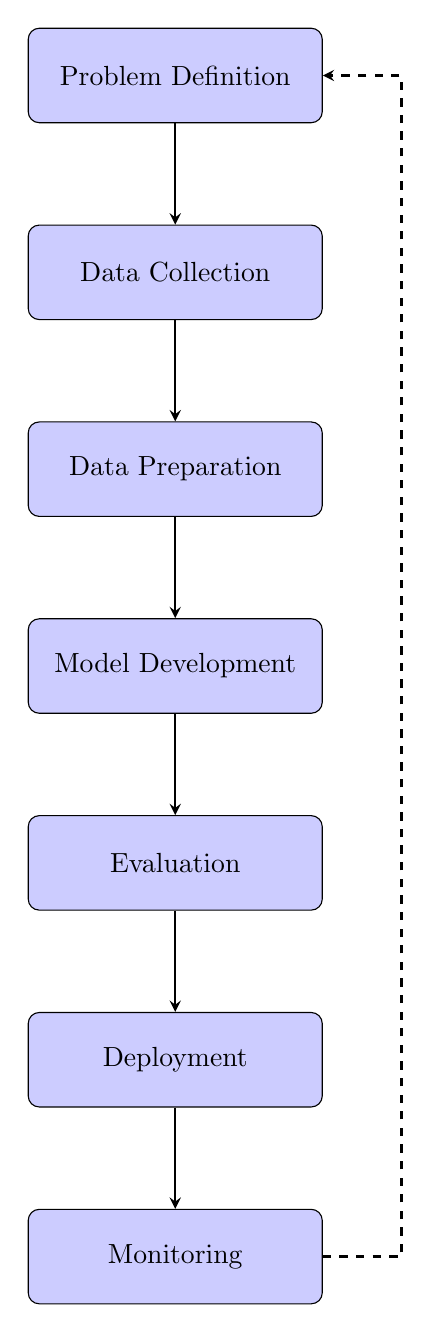
\begin{tikzpicture}[node distance=2.5cm]
    \tikzstyle{phase} = [rectangle, rounded corners, draw, fill=blue!20, text width=3.5cm, text centered, minimum height=1.2cm]
    \tikzstyle{arrow} = [thick,->,>=stealth]

    \node [phase] (problem) {Problem Definition};
    \node [phase, below of=problem] (data) {Data Collection};
    \node [phase, below of=data] (prep) {Data Preparation};
    \node [phase, below of=prep] (model) {Model Development};
    \node [phase, below of=model] (eval) {Evaluation};
    \node [phase, below of=eval] (deploy) {Deployment};
    \node [phase, below of=deploy] (monitor) {Monitoring};

    \draw [arrow] (problem) -- (data);
    \draw [arrow] (data) -- (prep);
    \draw [arrow] (prep) -- (model);
    \draw [arrow] (model) -- (eval);
    \draw [arrow] (eval) -- (deploy);
    \draw [arrow] (deploy) -- (monitor);
    \draw [arrow, dashed] (monitor.east) -- ++(1,0) |- (problem.east);
\end{tikzpicture}
\caption{The ML lifecycle with feedback loops}
\label{fig:ml_lifecycle}
\end{figure}

\section{Phase 1: Problem Definition}

\subsection{Framing the Business Problem}

The first phase establishes whether ML is appropriate for the problem and defines success criteria.

\begin{bestpractice}
Always start with the business problem, not the ML technique. Ask: "What decision will this model enable?" and "How will we measure success?"
\end{bestpractice}

Key activities include:
\begin{itemize}
    \item Defining the business objective and success metrics
    \item Determining whether ML is the right solution
    \item Assessing feasibility (data availability, timeline, resources)
    \item Establishing baseline performance
    \item Identifying stakeholders and requirements
\end{itemize}

\subsection{ML Problem Formulation}

Translate business objectives into ML problems:

\begin{itemize}
    \item \textbf{Classification:} Categorizing inputs into discrete classes
    \item \textbf{Regression:} Predicting continuous values
    \item \textbf{Ranking:} Ordering items by relevance
    \item \textbf{Clustering:} Discovering natural groupings
    \item \textbf{Anomaly Detection:} Identifying unusual patterns
\end{itemize}

\section{Phase 2: Data Collection and Understanding}

\subsection{Data Requirements}

Identify and acquire necessary data:

\begin{itemize}
    \item Define features and labels needed
    \item Assess data availability and quality
    \item Determine collection methods
    \item Consider privacy and legal constraints
    \item Plan for data versioning
\end{itemize}

\subsection{Exploratory Data Analysis}

Understand data characteristics:

\begin{lstlisting}[style=python]
import pandas as pd
import matplotlib.pyplot as plt
import seaborn as sns

# Load and inspect data
df = pd.read_csv('data.csv')
print(df.info())
print(df.describe())

# Visualize distributions
df.hist(figsize=(12, 10))
plt.tight_layout()
plt.show()

# Check for correlations
correlation_matrix = df.corr()
sns.heatmap(correlation_matrix, annot=True, cmap='coolwarm')
plt.show()

# Identify missing values
missing_data = df.isnull().sum()
print(missing_data[missing_data > 0])
\end{lstlisting}

\section{Phase 3: Data Preparation}

\subsection{Data Cleaning}

Address data quality issues:

\begin{itemize}
    \item Handle missing values (imputation or removal)
    \item Remove or correct outliers
    \item Fix inconsistencies and errors
    \item Deduplicate records
    \item Validate data integrity
\end{itemize}

\subsection{Feature Engineering}

Transform raw data into features:

\begin{lstlisting}[style=python]
from sklearn.preprocessing import StandardScaler, OneHotEncoder
from sklearn.compose import ColumnTransformer
from sklearn.pipeline import Pipeline

# Define transformations
numeric_features = ['age', 'income', 'credit_score']
categorical_features = ['city', 'occupation']

# Create preprocessing pipeline
preprocessor = ColumnTransformer(
    transformers=[
        ('num', StandardScaler(), numeric_features),
        ('cat', OneHotEncoder(drop='first'), categorical_features)
    ])

# Apply transformations
X_processed = preprocessor.fit_transform(X)
\end{lstlisting}

\section{Phase 4: Model Development}

\subsection{Model Selection}

Choose appropriate algorithms based on:

\begin{itemize}
    \item Problem type (classification, regression, etc.)
    \item Data characteristics (size, dimensionality, linearity)
    \item Performance requirements (accuracy, latency, interpretability)
    \item Resource constraints (computational budget, memory)
\end{itemize}

\subsection{Training and Validation}

Implement robust training procedures:

\begin{lstlisting}[style=python]
from sklearn.model_selection import train_test_split, cross_val_score
from sklearn.ensemble import RandomForestClassifier

# Split data
X_train, X_test, y_train, y_test = train_test_split(
    X, y, test_size=0.2, random_state=42, stratify=y
)

# Train model
model = RandomForestClassifier(n_estimators=100, random_state=42)
model.fit(X_train, y_train)

# Cross-validation
cv_scores = cross_val_score(model, X_train, y_train, cv=5)
print(f"CV Scores: {cv_scores.mean():.3f} (+/- {cv_scores.std():.3f})")
\end{lstlisting}

\section{Phase 5: Evaluation}

\subsection{Model Assessment}

Evaluate using appropriate metrics:

\begin{itemize}
    \item \textbf{Classification:} Accuracy, precision, recall, F1-score, ROC-AUC
    \item \textbf{Regression:} MAE, MSE, RMSE, R-squared
    \item \textbf{Ranking:} NDCG, MAP, MRR
\end{itemize}

\begin{lstlisting}[style=python]
from sklearn.metrics import classification_report, confusion_matrix
from sklearn.metrics import roc_auc_score, roc_curve

# Predictions
y_pred = model.predict(X_test)
y_pred_proba = model.predict_proba(X_test)[:, 1]

# Classification metrics
print(classification_report(y_test, y_pred))
print(confusion_matrix(y_test, y_pred))

# ROC-AUC
roc_auc = roc_auc_score(y_test, y_pred_proba)
print(f"ROC-AUC: {roc_auc:.3f}")
\end{lstlisting}

\section{Phase 6: Deployment}

\subsection{Deployment Strategies}

Choose deployment approach:

\begin{itemize}
    \item \textbf{Batch Prediction:} Process data in batches periodically
    \item \textbf{Online Prediction:} Real-time predictions via API
    \item \textbf{Edge Deployment:} Models running on devices
    \item \textbf{Hybrid:} Combination of approaches
\end{itemize}

\section{Phase 7: Monitoring and Maintenance}

\subsection{Production Monitoring}

Track key metrics:

\begin{itemize}
    \item Model performance metrics
    \item Prediction distribution
    \item Data drift detection
    \item System health (latency, throughput)
    \item Business impact metrics
\end{itemize}

\subsection{Model Maintenance}

Plan for ongoing maintenance:

\begin{itemize}
    \item Regular retraining schedule
    \item A/B testing new models
    \item Handling concept drift
    \item Updating features
    \item Documentation updates
\end{itemize}

\section{Iterative Nature of ML}

\subsection{Feedback Loops}

ML development is rarely linear. Common iteration points:

\begin{enumerate}
    \item Evaluation results prompt data collection or feature engineering
    \item Production monitoring reveals need for model updates
    \item Stakeholder feedback refines problem definition
    \item New data sources become available
\end{enumerate}

\section{Chapter Summary}

The ML lifecycle provides a framework for systematic ML development. Understanding each phase and their interconnections enables better planning, resource allocation, and risk management. Subsequent chapters will explore each phase in detail.

\section{Exercises}

\begin{exercise}
Map a familiar ML project to the lifecycle phases. Identify where iterations occurred and why.
\end{exercise}

\begin{exercise}
For a given business problem, work through the problem definition phase. Define success metrics and determine if ML is appropriate.
\end{exercise}
